\section{Durchführung}
\label{sec:Durchführung}
\subsection{Aufbau}
Der in diesem Versuch verwendete Aufbau ist in \autoref{fig:Aufbau} gegeben.
\begin{figure}
    \centering
    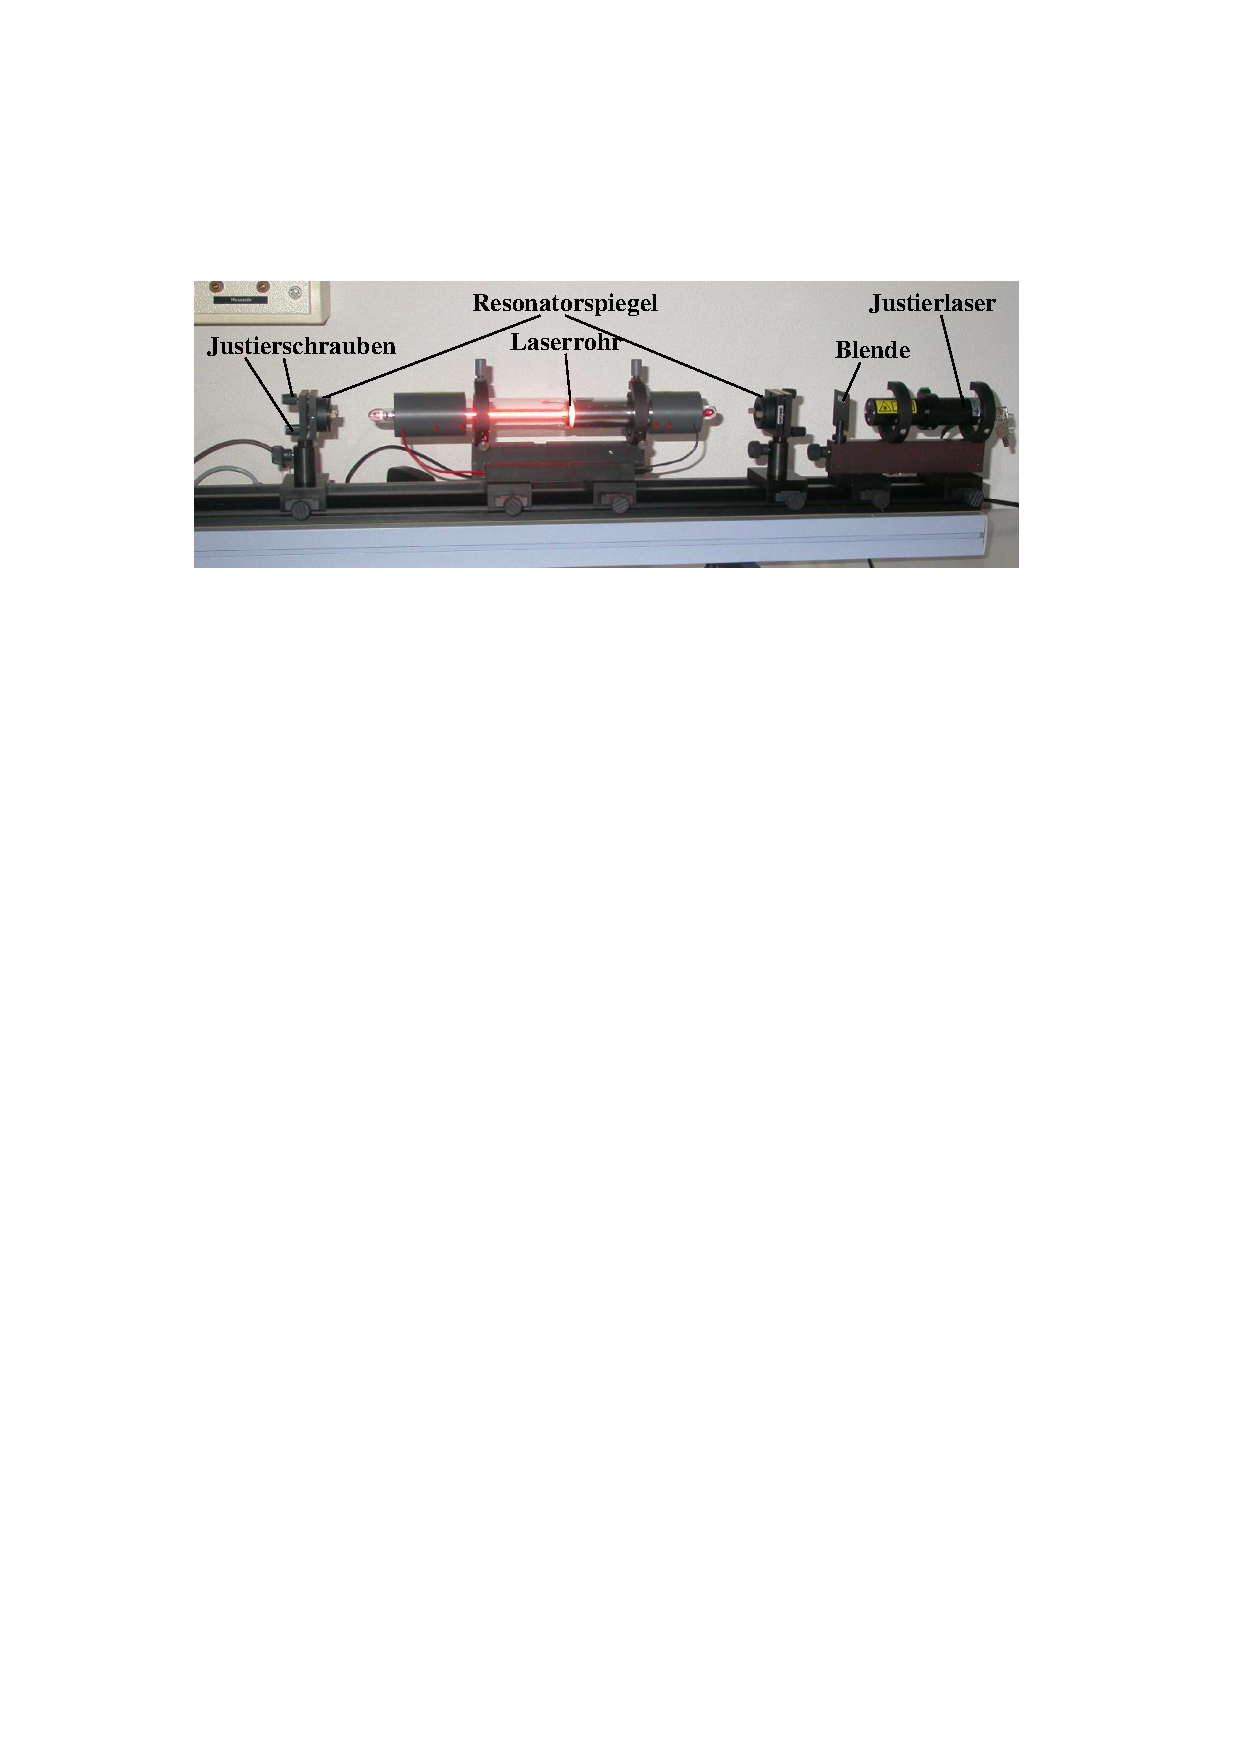
\includegraphics{content/pics/Aufbau.pdf}
    \caption{Foto des Versuchsaufbau. Auf einer optischen Schiene sitzen die einzelnen im Versuch benötigten Elemente \cite{v61}.}
    \label{fig:Aufbau}
\end{figure}
Auf einer optischen Schiene sind ein Justierlaser, das HeNe-Laserrohr mit eingebauten Brewsterfenstern, sowie Spiegel mit sehr hoher Reflektivität montiert.
Als Spiegel werden konkave oder planare Spiegel verwendet, wobei als Auskoppelspiegel nur ein konkaver Anwendung findet. Auf der optischen Schiene lassen sich alle
Elemente verschieben und in der Höhe verstellen. Außerdem können ein Intensitätsmessgerät, ein Polarisator, ein Frequenzanalysator, ein Gitter und ein Wolframdraht eingebaut 
werden.

\subsection{Überprüfung der Stabilitätsbedingung}
Zur Überprüfung der in \autoref{eq:g1g2} beschriebenen Stabilitätsbedingung wird für zwei verschiedene Spiegelkonfigurationen die Intensität
des Lasers in Abhängigkeit zu der Resonatorlänge gemessen. In diesem Versuch werden erst zwei konkave Spiegel mit einem Radius von 
$r=\qty{1400}{mm}$ und anschließend ein konkaver Spiegel mit demselben Radius und ein planarer Spiegel verwendet. Die Intensität wird 
jeweils mithilfe eines Intensitätsmessgerät bestimmt.

\subsection{Messung der Frequenzbreite}
Zur Messung der Frequenzbreite wird ein Frequenzanalysator verwendet, um in Abhängigkeit von der Resonatorlänge die jeweiligen 
Schwebungsfrequenzen zu bestimmen.

\subsection{Messung der TEM-Moden}
Damit TEM-Moden auf einem Schirm sichtbar werden, wird ein \qty{0.005}{\milli\metre} dünner Wolframdraht in den Resonator eingebaut.
Durch leichte Drehung des Drahts im Strahlengang werden verschiedene Moden sichtbar. Mithilfe einer Photodiode, welche auf einer zur optischen
Schiene senkrecht stehenden Schiene befestigt ist, wird die Intensitätsverteilung der Mode vermessen.

\subsection{Messung der Polarisation}
Die Polarisation des Laserlichts wird gemessen, indem ein Polarisationsfilter in den Laserstrahl eingebaut wird. Abhängig von der Drehung
des Polarisationsfilters wird abermals die Intensität bestimmt.

\subsection{Messung der Wellenlänge}
Zur Messung der Wellenlänge des Lasers wird das Licht an einem Gitter gebrochen. Der Abstand der dabei auftreten Intensitätsmaxima, sowie der Abstand des Schirms
zum Gitter werden dazu vermessen. 